% Straight up stealing preamble from Eli Holmes 
%%%%%%%%%%%%%%%%%%%%%%%%%%%%%%%%%%%%%%START PREAMBLE THAT IS THE SAME FOR ALL EXAMPLES
\documentclass{article}

%Required: You must have these
\usepackage{Sweave}
\usepackage{graphicx}
\usepackage{tabularx}
\usepackage{hyperref}
\usepackage{natbib}
\usepackage{pdflscape}
\usepackage{array}
\usepackage{gensymb}

%\usepackage[backend=bibtex]{biblatex}
%Strongly recommended
 %put your figures in one place
 
%you'll want these for pretty captioning
\usepackage[small]{caption}

\setkeys{Gin}{width=0.8\textwidth} %make the figs 50 perc textwidth
\setlength{\captionmargin}{30pt}
\setlength{\abovecaptionskip}{0pt}
\setlength{\belowcaptionskip}{10pt}
% manual for caption http://www.dd.chalmers.se/latex/Docs/PDF/caption.pdf

%Optional: I like to muck with my margins and spacing in ways that LaTeX frowns on
%Here's how to do that
 \topmargin -2cm     
 \oddsidemargin -0.04cm   
 \evensidemargin -0.04cm  % same as oddsidemargin but for left-hand pages
 \textwidth 16.59cm
 \textheight 22.94cm 
 %\pagestyle{empty}       % Uncomment if don't want page numbers
 \parskip 7.2pt           % sets spacing between paragraphs
 %\renewcommand{\baselinestretch}{1.5} 	% Uncomment for 1.5 spacing between lines
\parindent 0pt% sets leading space for paragraphs
\usepackage{setspace}
%\doublespacing

%Optional: I like fancy headers
\usepackage{fancyhdr}
\pagestyle{fancy}
\fancyhead[LO]{Phenological sequences}
\fancyhead[RO]{2017}

%%%%%%%%%%%%%%%%%%%%%%%%%%%%%%%%%%%%%%END PREAMBLE THAT IS THE SAME FOR ALL EXAMPLES

%Start of the document
\begin{document}

% \SweaveOpts{concordance=TRUE}
\bibliographystyle{/Users/aileneettinger/citations/Bibtex/styles/amnat.bst}
\title{Supplemental materials for \\ Phenological sequences: How early-season events define those that follow} 
\author{A.K. Ettinger, S. Gee, and E.M. Wolkovich}
%\date{\today}
\maketitle  %put the fancy title on
%\tableofcontents      %add a table of contents
%\clearpage
%%%%%%%%%%%%%%%%%%%%%%%%%%%%%%%%%%%%%%%%%%%%%%%%%%%
\renewcommand{\thetable}{S\arabic{table}}
\renewcommand{\thefigure}{S\arabic{figure}}


%\section*{Supplemental Methods}

%\section* {Supplemental Results}


%\section{Bibliography}
%\bibliography{/Users/aileneettinger/citations/Bibtex/mylibrary}

\section* {Supplemental Tables}

% latex table generated in R 3.4.2 by xtable 1.8-2 package
% Thu Feb  8 10:35:26 2018
\begin{table}[ht]
\centering
\caption{Summary of linear models for relationships between later phenophases and earlier phenophases, as shown in Figure 3 in the main text. Two types of linear models were fit: those with the intercept only estimated and a forced slope of one, and those with both the slope and intercept estimated (i.e. s standard regression model). All models were fit with the species-level mean day-of-year of the later phenological stages as the response variable, and mean day-of-year of earlier phenostage as the explanatory variable.} 
\label{table:prevphase}
\begin{tabular}{|p{0.27\textwidth}|p{0.07\textwidth}|p{0.05\textwidth}|p{0.05\textwidth}|p{0.07\textwidth}|p{0.05\textwidth}|p{0.05\textwidth}|p{0.07\textwidth}|p{0.05\textwidth}|}
  \hline
  &\multicolumn{3}{c |}{forced slope model} &\multicolumn{5}{c |}{standard regression model}\\
 \hline previous phenostage model & intercept & r\textsuperscript{2} & aic & intercept & slope  & p & r\textsuperscript{2} & aic \\
 \hline
leafout vs. budburst & 8.94 & 0.10 & 164.78 & 65.84 & 0.53 & <0.001 & 0.44 & 155.01 \\ 
  flowering vs. budburst & 23.83 & 0.17 & 225.55 & 3.18 & 1.17 & 0.039 & 0.17 & 227.45 \\ 
  fruiting vs. budburst & 46.87 & 0.17 & 246.71 & -80.31 & 2.04 & 0.016 & 0.23 & 246.87 \\ 
  senescence vs. budburst & 158.84 & -0.12 & 210.97 & 243.88 & 0.30 & 0.427 & 0.03 & 209.43 \\ 
  flowering vs. leafout & 14.90 & 0.23 & 223.60 & -105.28 & 1.92 & 0.005 & 0.30 & 223.26 \\ 
  fruiting vs. leafout & 37.93 & 0.11 & 248.29 & -107.19 & 2.11 & 0.051 & 0.16 & 249.05 \\ 
  senescence vs. leafout & 149.90 & -0.07 & 209.74 & 237.39 & 0.33 & 0.484 & 0.02 & 209.58 \\ 
  fruiting vs. flowering & 23.04 & 0.54 & 232.14 & 5.21 & 1.12 & <0.001 & 0.54 & 233.79 \\ 
  senescence vs. flowering & 135.00 & -1.79 & 233.74 & 261.65 & 0.13 & 0.332 & 0.04 & 209.08 \\ 
  senesence vs. fruiting & 111.97 & -5.43 & 254.66 & 277.81 & 0.02 & 0.851 & 0.00 & 210.09 \\ 
   \hline
\end{tabular}
\end{table}% latex table generated in R 3.4.2 by xtable 1.8-2 package
% Thu Feb  8 10:35:27 2018
\begin{table}[ht]
\centering
\caption{Summary of linear models for relationships between later phenophases and interphase duration, as shown in Figure 4 in the main text. Linear models were fit with the species-level mean day-of-year of the later phenological stages as the response variable, and the number of days in each previous interphase duration as the explanatory variable.} 
\label{table:interphase}
\begin{tabular}{|p{0.35\textwidth}|p{0.1\textwidth}|p{0.07\textwidth}|p{0.07\textwidth}|p{0.07\textwidth}|p{0.07\textwidth}|}
  \hline
interphase model & intercept & slope & r\textsuperscript{2} & p & aic \\ 
  \hline
leafout vs. leafout-budburst & 128.98 & 0.20 & 0.04 & 0.374 & 168.58 \\ 
  flowering vs. leafout-budburst & 144.52 & 0.12 & 0.00 & 0.874 & 232.14 \\ 
  fruiting vs. leafout-budburst & 276.48 & -1.56 & 0.05 & 0.3 & 264.61 \\ 
  senescence vs. leafout-budburst & 281.98 & -0.15 & 0.00 & 0.763 & 210.03 \\ 
  flowering vs. flowering-leafout & 129.28 & 1.10 & 0.93 & <0.001 & 167.11 \\ 
  fruiting vs. flowering-leafout & 245.86 & 1.12 & 0.25 & 0.011 & 245.86 \\ 
  senescence vs. flowering-leafout & 278.63 & 0.13 & 0.03 & 0.381 & 209.27 \\ 
  fruiting vs. fruiting-flowering & 143.56 & 1.02 & 0.74 & <0.001 & 232.15 \\ 
  senescence vs. fruiting-flowering & 258.29 & 0.19 & 0.24 & 0.013 & 203.20 \\ 
  senesence vs. senescence-fruiting & 282.11 & -0.08 & 0.05 & 0.296 & 208.91 \\ 
   \hline
\end{tabular}
\end{table}\clearpage

\section* {Supplemental Figures}

\begin{figure}[h]
  \centering
  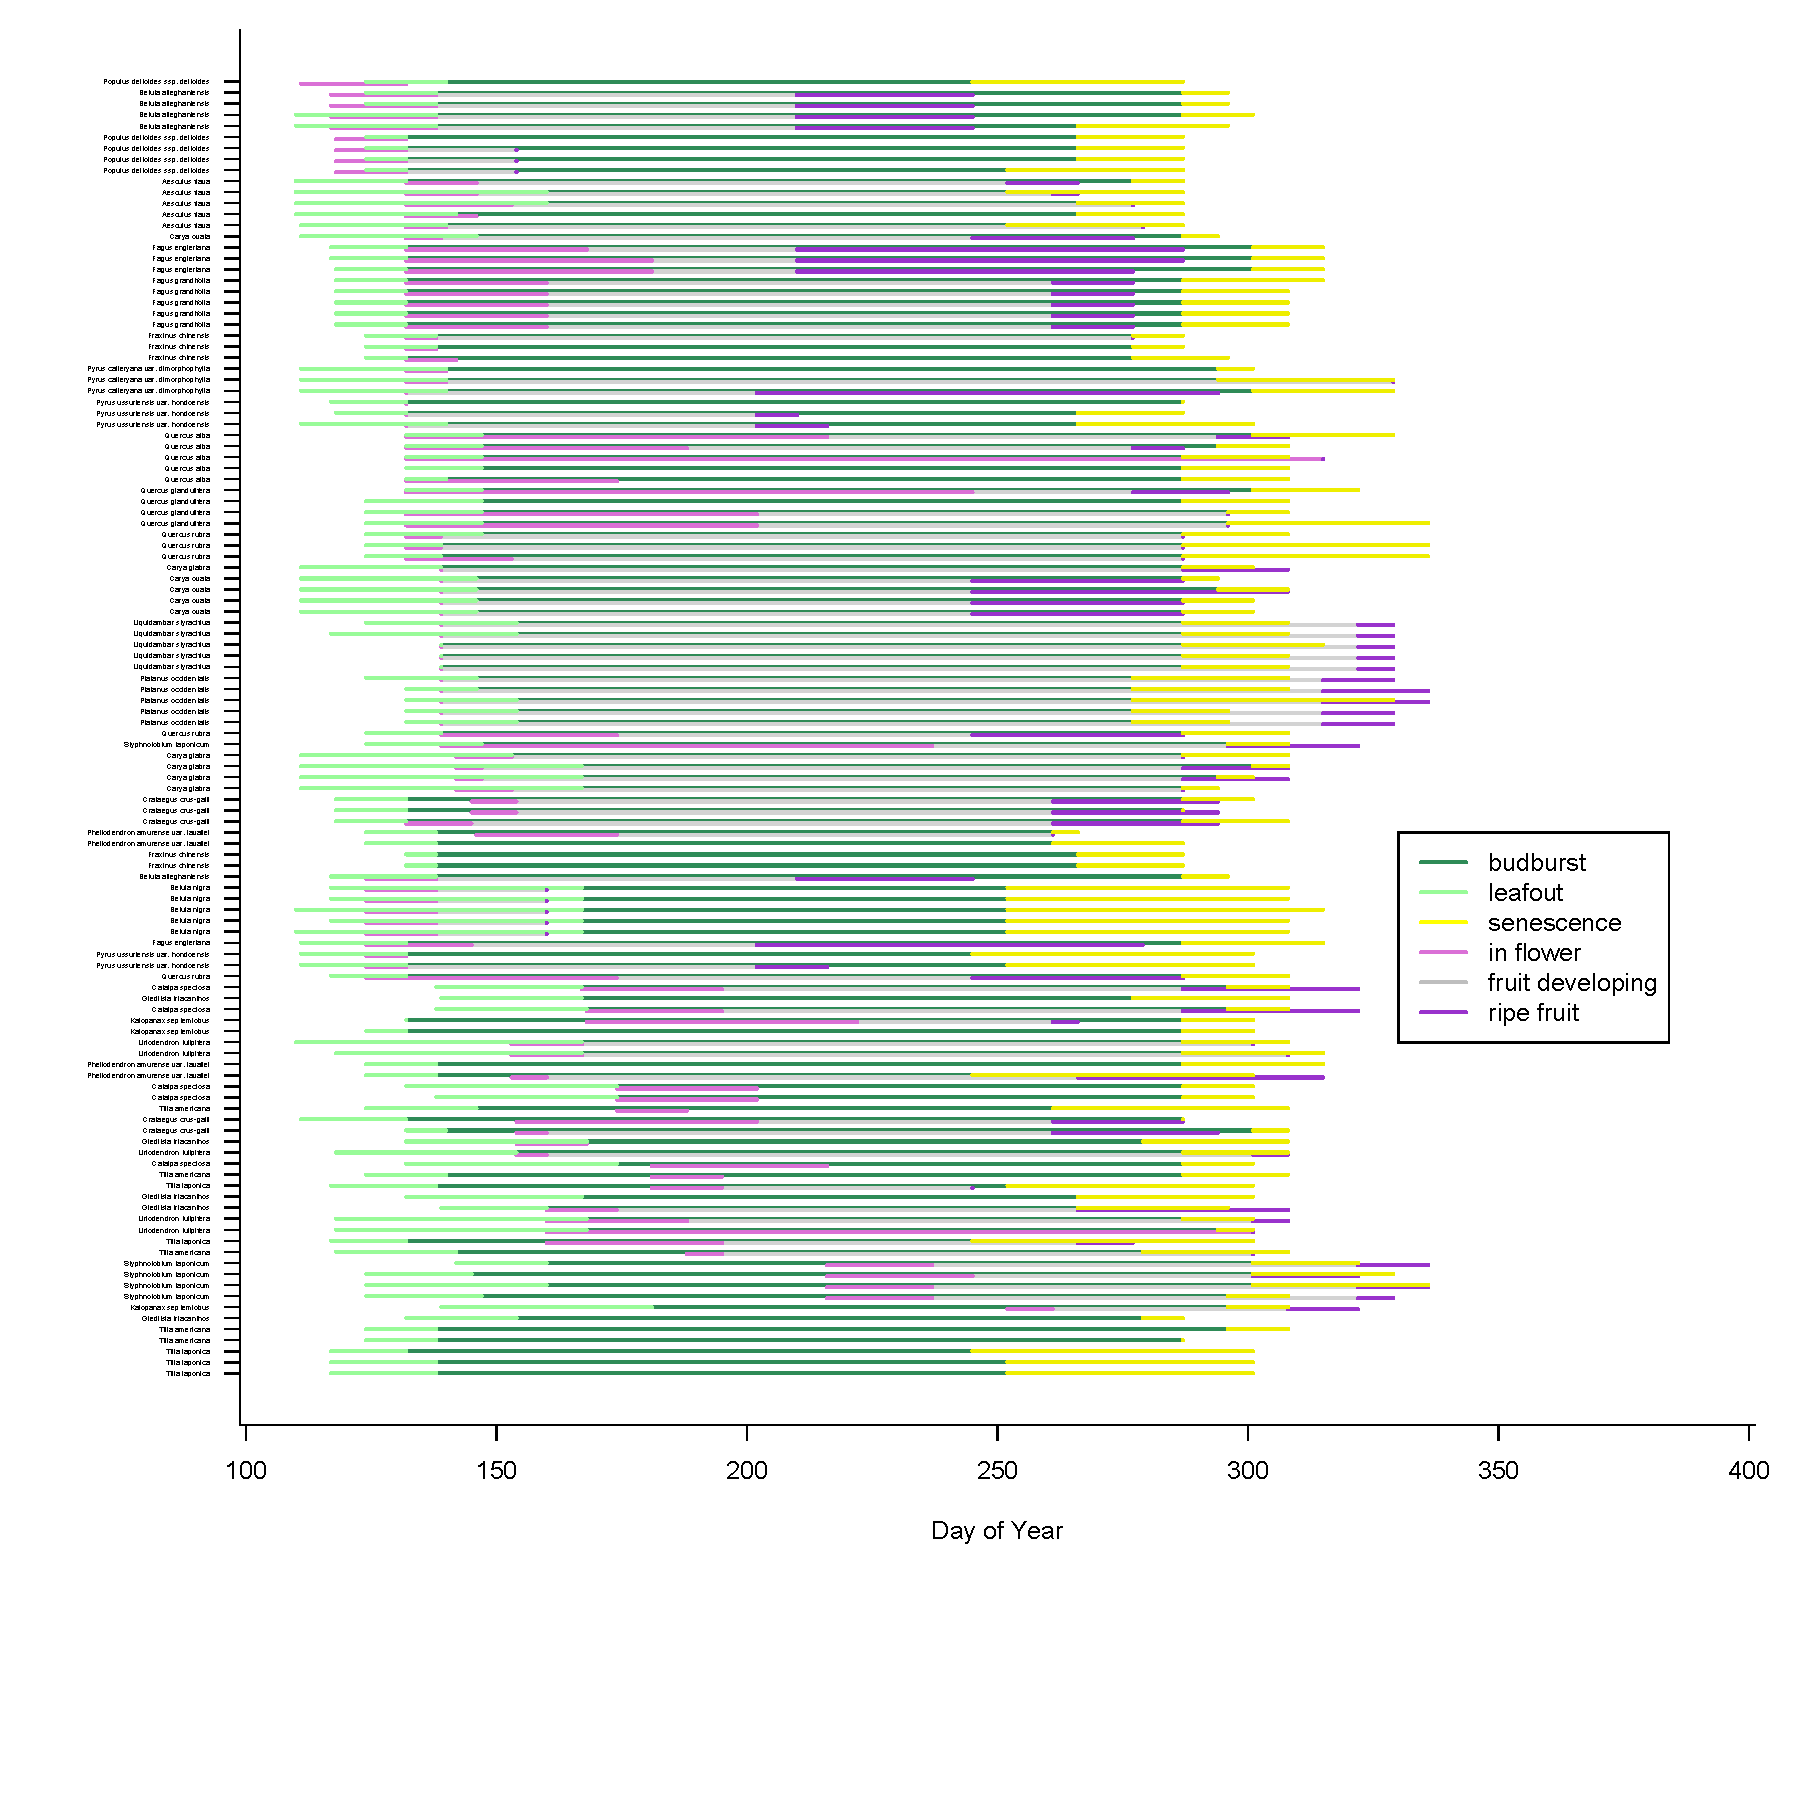
\includegraphics{../analyses/figures/grosea_repsort_ripefruit_ind_legend.pdf}
  \caption{\textbf{Individual tree phenology during the 2015 growing season, ordered by species-level mean first-flower dates.} Growth phenology is shown for budburst (from its mean start day-of-year to the mean start day-of-year for leafout, across all individuals within a species), leafout (from the mean day-of-year when fully-expanded leaves were first observed through the start of senescence), and senescence (from the mean day-of-year when leaves first began changing color through the mean day-of-year when more than 95 percent of leaves on the tree had changed color). Reproductive phenology is shown for flowering (from the mean day-of-year when flowers first appeared to the mean day-of-year when fruits first appeared, across all individuals within a species) and fruiting (from the mean day-of-year when fruits first appeared to the mean day-of-year when more than 95 percent of fruits were first observed as ripe).}
 \label{fig:focind}
\end{figure}
  
%%%%%%%%%%%%%%%%%%%%%%%%%%%%%%%%%%%%%%%%
\end{document}
%%%%%%%%%%%%%%%%%%%%%%%%%%%%%%%%%%%%%%%%
